%! Author = erick-hdz
%! Date = 15/05/20

% Preamble
\documentclass[10pt]{report}


% Packages
\usepackage{blindtext}
\usepackage{amsmath}
\usepackage[utf8]{inputenc}
\usepackage[spanish]{babel}
\usepackage{fancyhdr}
\usepackage{graphicx}
\usepackage{algorithm, algorithmic}
\usepackage{amsfonts}
\usepackage{amsbsy}
\usepackage{makeidx}
\usepackage{geometry}
\usepackage{listings}
\usepackage[T1]{fontenc}
\usepackage{natbib}
\usepackage{amsthm}
\usepackage{amssymb}
\usepackage{lastpage}
\usepackage{multicol}
\usepackage{xcolor}
\usepackage{glosmathtools}

%Status of the document

\pagenumbering{roman}
\newtheorem{example}{Example}
\newtheorem{corrollary}{Corrollary}
\newtheorem*{remark}{Remark}
\newtheorem{definition}{Definition}
\newtheorem{theorem}{Theorem}
\pagestyle{fancy}
\fancyhf{}
\rhead{Sección de tesis}
\lhead{Simulación de modelos}
\rfoot{Page  \thepage}
\author{Erick Hernandez Navarrete}
\title{Simulación de modelos}


% Document
\begin{document}
    %todo:Correcciones del documento en forma de check speller
    %todo:Hacer antes de esta semana lo antes posible
    %todo:puntear a manera de commit los elementos del Cap 1
    %TODO:Hacer las correcciones de al menos el primer capitulo de la tesis
    \maketitle
    \tableofcontents{}
    \chapter{Decidibilidad en los modelos}\label{ch:decidibilidad-en-los-modelos}
    \section{Introducción}\label{sec:introducción}
    En este documento se expondrán las nociones de decibilidad, complejidad en ambos modelos %Add complexity part of both worlds
    en el mundo de máquinas de Turing y en el mundo distribuido,
    así como también se hará la formalización de la noción de simulación de modelos
    computacionales, demostrando que el modelo $A$ de  la máquina de
    Turing es equivalente en poder al modelo distribuido $B$, en particular al modelo \textbf{LOCAL}

    \section{Decidibilidad del modelo máquinas de Turing}\label{sec:decidibilidasd-en-el-modelo-de-máquinas-de-turing}
    %!todo:Hacer una explicacion intuitiva de lo que es una máquina de Turing,despues de esta done
    %!todo: de esta explicación intuitiva
    %!todo: Hacer un feedback con la escritura para que se pula la parte de la gramática


    \subsection{Cadenas y lenguajes}\label{sec:Cadenas-y-lenguajes}
    Ahora, se definirán los bloques constructores de ciencias de la computación, es decir las cadenas de carácteres.
    Con el propósito de definir lo siguiente:\space
    \begin{definition}
            Decimos que un alfabeto es cualquier conjunto $X$ tal que $X != \emptyset$
    \end{definition}
    \newline
    Una vez que se define el concepto de alfabeto, los elementos del lenguaje son los símbolos del alfabeto.
    Se estipulará que las letras mayúsculas se usarán para los alfabetos y letras minúsculas para los símbolos.
    En virtud de ello se pude enuciar algunos ejemplos de alfabetos:
    \begin{itemize}
        \item $\Theta_{1} = \{0,1,2,3,4,5,6,7,8,9 \}$
        \item $\Theta_{2} = \{a,b,c,d,e,f,g,h,i,j,k,l \}$
        \item $\Omega = { 0,1,x,y,z,t}$
    \end{itemize}\space
    Lo siguiente es definir la noción de una cadena sobre un alfabeto, que para los fines de este estudio
    son los bloques constructores del mismo, y que son, al mismo tiempo, en el modelo de
    máquinas de Turing las entradas de instancias de este modelo, lo que dará la noción de cómputo.
    \begin{definition}
        Una \textbf{cadena} sobre un alfabeto $\Sigma$ es una secuencia finita de símbolos del alfabeto,
       que es usualmente escrito cada símbolo uno sobre otro y sin separación por comas.
    \end{definition}
    Una vez que se tiene la noción de cadena sobre un alfabeto, se puede dar unos cuantos ejemplos:
    \begin{itemize}
        \item Si $\Sigma_{1} = \{a,b\}$, entonces la cadena $abbaba$ es una cadena sobre $\Sigma_{1}$
        \item Si $\Sigma_{2} = \{ 2,3,5 \}$, entonces la cadena $32225$ es una cadena sobre $\Sigma_{2}$
    \end{itemize}
    Entonces ahora que se definió el concepto cadena sobre un alfabeto podemos definir atributos a las cadenas definidas sobre un
    alfabeto $\Sigma$,\newline
    \begin{definition}
        Sea $w$ una cadena sobre un alfabeto $\Sigma$,dicha cadena tiene \textbf{longitud},
        y se denotorá como $|w|$, y asi se concluirá que es el número de símbolos que contiene.

    \end{definition}
    Entonces con base a esa definición, se denominará vacía a la cadena tal que su longitud es cero, y la
    distinguiremos como $\epsilon$.\newline
    Se puede escribir a una cadena $w = w_{1},\mathellipsis w_{n}$, sobre un alfabeto $\Sigma$ si cada $w_{i} \in \Sigma$;
    \space
    A continuación se definirán ciertas operaciones o atributos asociados a estas estructuras de datos.
    \begin{definition}
        Sea una cadena $w$, se asociará a la cadena $w$ la cadena reversa denotada como $w^R$
        y con la notación, si $w = w_{1},\mathellipsis w_{n}$, entonces $w^{R} = w_{n},\mathellipsis,w_{1}$.
    \end{definition}
    También se dará la noción de sub-cadena, la cual enunciaremos de la siguiente manera:\newline
    \begin{definition}
        Sean $z,w$ cadenas, se puede decir que $z$ es una sub-cadena de $w$ si aparece de manera consecutiva dentro de $w$.
    \end{definition}
    Ejemplos de subcadenas son:
    \begin{itemize}
        \item $abc$ es una sub-cadena de la cadena $abcdedfg$
        \item $cdcd$ es una subcadena de la cadena $cdasdcadccdcd$
    \end{itemize}
    También se definirá una operación entre dos cadenas, la cual es
    la concatenación, entonces se define formalmente de la siguiente manera:\newline
    \begin{definition}
        Sean $w_{1}$ y $w_{2}$ dos cadenas finitas, esto es:\newline
        $\exists n,\ \exists m$ tal que $|w_{1}|=n$ y $|w_{2}|=m$
        entonces la cadena $r = w_{1}w_{2}$, es el resultado de agregar la cadena $w_{2}$ al final de la cadena
        $w_{1}$.\newline
        En notacion es: $concat(w_{1},w_{2}) = w_{1}w_{2}$
    \end{definition}
    Entonces con esta definición de operación se hará el equivalente en potencia en matemáticas,
    formalmente lo podemos decir:\newline
    \begin{definition}
        Sea $x$ una cadena sobre un alfabeto $\Sigma$, entonces concatenar dicha cadena
        $m-veces$, con $m\in\N$ se escribirá así:\newline
        $x\dots x = x^m$
    \end{definition}
    Finalmente se tiene la noción universo de las cadenas para algún alfabeto, que se formalizará de la
    siguiente manera:
    \begin{definition}
        Sea un alfabeto $\Sigma$, se dice que un lenguaje es un conjunto de cadenas sobre el alfabeto $\Sigma$, i.e
        \begin{equation}
            \label{eq:equation7}
             L = \{w : w\ es \ una \ cadena\ sobre \Sigma \}
        \end{equation}
    \end{definition}
    Entonces, una vez que se tiene la definición de lenguaje, lo siguiente es presentar el modelo de máquina de Turing,
    ya que en este contexto los problemas se modelarán en términos de lenguaje, con la noción anteriormente anunciada.
    \newline

    \subsection{Elementos del modelo}\label{subsec:elementos-del-modelo-de-máquina-de-turing}
    Ahora, se dará la definición del modelo formal de computo, a saber el modelo de máquina de Turing,
    para ello se tendrá una presentación intuitiva del modelo.\newline
    El modelo de máquina de Turing es a grandes razgos un modelo con cierta robustez; lo cual quiere decir que se tendrá la posiblidad
    de resolver una cantidad de problemas, pero con ciertas limitantes.
    \newline

    Este modelo fue propuesto por primera vez en 1936 por el matemático \textbf{Alan Turing}, similares a
    otros modelos de cómputo que no se presentará en esta tesis, como son solo por decir: autómatas finitos.
    El modelo de máquina de Turing usa una cinta infinita como su memoria ilimitada,
    además tine el cabezal, que es la que permité leer y escribir símbolos además de moverse
    a lo largo de la cinta.
    \newline
    Inicialmente la cinta contiene únicamente como entrada a la cadena, y lo demás es blanco.
    Si la máquina necesita almacenar información, esta tendrá que ser escrita en la cinta.\newline
    Para leer la información que ha sido escrita en la cinta esta tendrá que mover su cabezal sobre ella.\space
    La máquina continurá computando hasta que tenga una salida, lo que se traduce a que tendrá una sucesión de pasos
    como los que se describieron anteriormente, hasta que se dé la definición formal de la palabra cómputo.
    \newline

    Las salidas: aceptación, rechazo, se obtienen una vez que se ha entrado en los estados de aceptacion, rechazo,
    por otro lado si no entrá en alguno de los estados que se mencionaron anteriormente, la máquina continurá para siempre, i.e
    ésta nunca terminará de hacer su cómputo.\newline
    Esta es la presentación intuitiva de este modelo, entonces lo que sigue es definir de manera formal los elementos del modelo,

    \newline

    \begin{definition}%!Here we need to rewrite for errors
        Una máquina de Turing is una 7-tupla, $(Q,\Sigma,\Lambda,\delta,q_{0},q_{accept},q_{reject})$
        donde $Q,\Sigma,\Lambda$ son conjuntos finitos.
        \begin{enumerate}
            \item $Q$ es el conjunto de estados,
            \item $\Sigma$ es el alfabeto de entrada que no contiene el símbolo blanco $\sqcup$
            \item $\Lambda$ es el alfabeto de la cinta donde  $\sqcup\in\Lambda$ y además $\Sigma\subseteq\Lambda$,
            \item $\delta: Q\times\Lambda \rightarrow Q\times\Lambda\times\{L,R,S\}$ es la función de transición
            \item $q_{0}$ es el estado de iniciación,
            \item $q_{accept}$ es el estado de aceptacion
            \item $q_{reject}$ es el estado de rechazo donde $q_{accept} \neq q_{reject}$,

        \end{enumerate}
        Aquí los símbolos $L,R,S$ son el imperativo para el movimiento del cabezal \textbf{Left}, \textbf{Right} y \textbf{Stay}
    \end{definition}
    Una vez que se tiene la definición se presentará como es el cómputo:\newline
    Inicialmente, se tendrá como entrada una cadena $w = w_{1}\dots w_{n}$ en $\Sigma$, en a lo más $n$ cuadros
    a la izquierda y el resto de la cinta esta en blanco.Ésto quiere decir que están rellenados con símbolos blancos,
    y la manera de identificar el final de la entrada $w$ es marcado por el primer símbolo en blanco en la cinta,
    ya que el alfabeto $\Sigma$ no contiene dicho símbolo.
    \newline

    Luego, una vez que inicia la máquina $M$ con la entrada $w$, el cómputo estará gobernado por la función $\delta$.
    Algo que se puede observar es que si en algún momento del cómputo el cabezal intenta moverse a la izquierda del lado
    izquierdo extremo, éste se quedará en el mismo lugar, aunque la función de transición indique un movimiento del cabezal $L$.
    \newline

    Finalmente, el cómputo continuará hastá que entre en el estado de $q_{accept}$ ó $q_{reject}$,
    si no sucede lo anterior $M$ continuará para siempre.
    Una vez presentado el modelo y una visión intuitiva del cómputo en el mismo, se adentrará a la noción de
    \textbf{decidible}, que es la noción a la que se quiere converger en este modelo para hacer la conexión con el modelo
    de cómputo distribuido.

    \newline
    %!todo:Definir como se estan resolviendo los problemas en el contexto de maquinas de Turing
    %!todo:Esto quiere decir que es un lenguaje etc.
    %!Final de las observaciones de la edicion de este capitulo.
     \subsection{Decidibilidad}\label{subsec:decidibilidad2}
    Ahora la noción de \textbf{configuración} es lo que nos permitirá formalizar el movimiento del
    cabezal de la máquina, que esto en esencia será la formalización del cómputo en este modelo.
    \newline
    La manera en que $M$ hace el compúto, de manera intuitiva se puede decir que ocurren ciertos eventos, a saber:
    \begin{itemize}
        \item Cambio en el estado actual
        \item Cambio en el contenido de la cinta
        \item Cambio en la localidad del cabezal
    \end{itemize}
    Estos eventos se constituirán al definir el término configuración.
    Los elementos serán en esencia tomarse el estado actual, digamos $q_{a}$, el contenido actual de la cinta, por ejemplo:
    $uv$ con $u,v$ cadenas para el alfabeto $\Sigma$ y la localidad actual de la cinta, que será el primer
    símbolo de la cadena $v$. \newline
    Esto se puede plantear en la triada:
    \begin{equation}
        C = (u,q,v)
    \end{equation}
    Con $u,v$ cadenas y $q$ es el estado actual, y la posición actual es el primer símbolo de la cadena $v$,
    en este sentido se puede escribir de la siguiente manera esta noción:
    \begin{equation}
        uqv
    \end{equation}
    Para enfatizar que en ese momento del compúto, el cabezal esta en la localidad del primer símbolo de la cadena
    $v$, se coloca a el estado actual $q$ entre la cadena $u$ y $v$; esto da un significado formal a la notación del concepto
    de configuración.
    \\
    \newline
    Entonces esta noción es la que va a dar el paso de formalizar el compúto, por lo cual de manera intuitivamente se va
    a tener una secuencia de configuraciones:\newline
    \begin{equation}
        C_{0}\mathellipsis C_{n}\in\mathbb{N}
    \end{equation}
    \newline

    Pero este proceso se definirá entre dos estados a priorí $C_{i},C_{j}$;
    entonces esta noción permitirá definir lo siguiente:
    \begin{definition}
        Se dice que la \textbf{configuración} $C_{j}$ le sigue a $C_{k}$ si:
        Se toman las cadenas $u,v$ de $\Gamma$, y también tomamos $a,b\in \Sigma$.
        entonces se concluye que: si pasa $\delta(q_{k},b) = (q_{j},c,L)$,
        entonces $uacq_{j}v$ le sigue de $uaq_{k}bv$

    \end{definition}
    La anterior noción se esta definiendo con la función $\delta$, que es la que esta formalizando esta noción.
    Como se menciono anteriormente, se estipula que las secuencias de configuraciónes, entonces se tendrá una configuración
    inicial.
    \begin{definition}
        Sea $M$ una máquina de Turing, $w$ una cadena, tomamos a
         la configuracion inicial $C_{0}$, y se representa con base a lo anterior como $q_{0}w$
        \end{definition}
    \newline
    El significado de la notación de la configuración inicial es que esta en
    el estado cero $q_{0}$ y el cabezal esta en el primera localidad de lado izquierdo de la cinta.
    Ahora las configuraciones que intuitivamente son las candidatas para
    que sean las configuraciones finales si es que la máquina termina en algun momento de este
    proceso; pero por el momento se llamará a esas configuraciones:\newline
    \begin{equation}
        q_{accept}, q_{reject}\label{eq:equation8}
    \end{equation}
    A estas configuraciones se les nombrarán como configuraciones de paro, ya que están definidas
    en términos del estado en el que entran; que son los estado de paro y de aceptación respectivamente.\newline
    %TODO: Hacer una revisión gramatical de la tesis
    Entonces se formalizará que una máquina de Turing se detiene si entra en los estados
    $q_{accept0},q_{reject}$ y con base a esto se hará una generalización de la definición de la función delta, tomando
    un conjunto de estados en el que no esta los estado de detención
    \newline
    Una vez aclarado esto, se tienen los elementos para definir que:\newline
    Dada una máquina $M$ acepta a una
    cadena arbitraria $w$.  
    \begin{definition}
        Sea una cadena $w$ y una máquina de Turing $M$,\newline
        entonces se dice que $M$ acepta a la cadena $w$ si:
        \begin{enumerate}
            \item $C_{1}$ es la configuración inicial con entrada $w$
            \item cada $C_{i+1}$ le sigue de $C_{i}$
            \item existe un $k \in \N$ tal que $C_{k}$ es una configuración de aceptación
        \end{enumerate}
    \end{definition}
    %! Esta es una descripción a un alto nivel de estos objectos formale
    Esto esta formalizando la noción de que una máquina de Turing \textbf{acepta} a una cadena $w$
    y lo que se observa es que los problemas que se plantean, se
    escriben en términos del lenguaje, es decir, el sentido formal de lenguaje; que son los
    conjuntos de cadenas formadas sobre un alfabeto dado $\Sigma$.
    \newpage
    En este sentido, dada una máquina de Turing $M$,se puede tener la "coleccióń" de todas
    las cadenas que son aceptadas por $M$, que con base a la definición de lenguaje en el mundo de máquinas de Turing
    esto es el conjunto de cadenas con el atributo de que son aceptadas por $M$, sobre un alfabeto $\Sigma$.
    \newline
    Ahora se formalizara lo anterior de la siguiente manera:
    \begin{definition}
        Sea $M$ una máquina de Turing, al conjunto de cadenas $w$ que son aceptadas por $M$ sobre el alfabeto $\Sigma$,
        se llamarán el lenguaje que \textbf{reconoce} $M$, se escribirá como $L(M)$.

    \end{definition}
    \newline
    Ahora con estas definiciones, se tendrá la siguiente noción: \newline Sea $L$ un lenguaje sobre un alfabeto $\Sigma$,
    se estipulará en términos de la existencia de una máquina de Turing que lo hace reconocible;
    así se formalizará de la siguiente manera: \newline
    %Todo: Hacer las correcciones de edicion de las partes faltantes para concluir esta parte correspondiente

    \begin{definition}
        Sea $L$ un lenguaje, se dice que es Turing-reconocible si:
        existe una máquina de Turing que lo hace Turing-reconocible.
    \end{definition}

    \begin{remark}
        Cuando se inicia una máquina de Turing con entrada $w$, pasan tres posibles eventos:
        \begin{itemize}
            \item acepta,
            \item rechaza,
            \item nunca se detiene.
        \end{itemize}
    \end{remark}
    %!Aqui vamos a hacer el enfasis de que siempre tendremos maquinas que paren.
    En este caso, se tomará solamente máquinas de Turing que se detienen en algun momento en la ejucución para todas sus entradas,
    por lo tanto en términos formales, dichas máquinas siempre se dentendrán en algún momento de la
    ejecución de $M$, para $\forall w$ entrada.
    Se formalizará lo anterior con una definición.
    \begin{definition}
        Sea $M$ máquina de Turing tal que $\forall w$ entrada, si esta se detiene en algún momento de la ejecución,
        entonces dicha máquina de Turing tiene el atributo de ser
        \textbf{decidible}\newline
        Donde $w$ es una cadena sobre el alfabato $\Sigma$
        Es decir, siempre entrán en su estado de \textbf{aceptación}
        o en su estado de \textbf{rechazo} en algún momento de la ejecución.
    \end{definition}
    Y por el lado de la noción del lenguaje definimos lo siguiente:
    \begin{definition}
        Se dicé que un lenguaje es \textbf{decidible} si existe un máquina de Turing
        que lo \textbf{decide}.
        i.e que la máquina tiene el atributo de ser decidible.
    \end{definition}
    %!Exponer un ejemplo de máquina de Turing, tanto en esta version, como en la versión final de esta tesis
    Una vez que se tiene el concepto de máquina de Turing, daremos un ejemplo de un lenguaje que es decidible,
    i.e expondremos una máquina de turing \textbf{decidible}.

    \begin{example}
        Tomamos el siguiente lenguaje:
        \begin{equation}
            A = \{ 0^2^n : n>=0\}\label{eq:equation2}
        \end{equation}
        Es el lenguaje que consta de cadenas de 0's tal que su longitud es una
        potencia de 2.
    \end{example}
    Entonces se afirma que $M_{2}$ es un lenguaje decidible.
    %!Hacer un sketch de que es un lenguaje decidible
    Entonces se puede hacer las instrucciones (alto  nivel) para $M_{2}$ como sigue:
    \begin{enumerate}
        \item Recorrer de izquierda a derecha a través de la cinta, tachando uno de cada dos ceros
        \item Si en la etapa 1, la cinta contenia un solo $0$, entonces \textbf{acepta}
        \item Si en la etapa 1, la cinta contenía mas de un $0$ y además un número impar, mayor a $1$, \textbf{rechaza}
        \item Regresa el cabezal al lado izquierdo al final de la cinta
        \item Ve a la etapa 1
    \end{enumerate}
    Una vez que se tiene la descripción de la máquina de Turing a un alto nivel, se puede hacer un puente
    a un bajo nivel, que es formalmente describir la máquina con sus elementos que la definen para una entrada $w$,
    el cual nuestro puente será en describir la función $\delta$ vía un diagrama de estados
    %!Describiendo el alto nivel de la maquina de Turing a un alto nivel.
    En la etapa 1 de $M_{2}$, corta el número de ceros a la mitad. Mientras la máquina barre tráves de la cinta en la
    etapa 1, lleva la cuenta de $0$'s vistos si es par o impar.\newline Si el número es impar mayor a 1, entonces el número original
    de $0$'s en la entrada no puede ser una potencia de 2. Entonces la máquina \textbf{rechaza} en esa instancia.
    Si el número de 0's visto es 1, entonces el número original tiené que ser una potencia de 2, entonces en ese
    caso la máquina \textbf{acepta}.
    %!Descripción formal de la máquina de Turing.
    Sea $M_{2} =(Q,\Sigma,\Lambda,\delta,q_{1},q_{accept},q_{reject})$:
    \begin{enumerate}
        \item $Q = \{q_{1},q_{2},\dots,q_{5},q_{accept},q_{reject}$,
        \item $\Sigma = \{ 0 \}$ and
        \item $\Lambda = \{0,x,\sqcup \}$.
        \item Se describirá a $\delta$ con un diagrama de estado.
        \item Los estados de inicio, aceptación y rechazo son $q_{1},q_{accept},q_{reject}$ respectivamente.
    \end{enumerate}
    \newline
    %!Todo: Hacer el diagrama de estado para que sea una mejor presentación.
    %!Este diagrama se hara de la manera de draw.io

    \begin{center}
        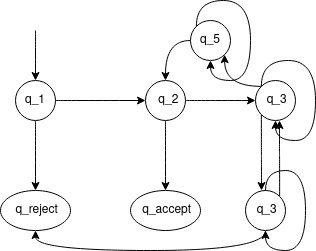
\includegraphics{Untitled Diagram.jpg}
    \end{center}
    \newline
    En este diagrama, la etiqueta $0\rightarrow \sqcup,R$ que muestra en la transición del estado $q_{1}$ al estado $q_{2}$,
    tiene la semántica de la definición de la función $\delta$, que en otras palabras se describe como si:\newline
    en el estado $q_{1}$ con el cabezal leyendo $0$, la máquina va al estado $q_{2}$, escribe $\sqcup$ y mueve el cabezal
    a la derecha.\newline
    Lo que en términos formales significa que: $\delta(q_{1},0) = (q_{2},\sqcup, R)$.
    Otra escritura que se usará para la notación en este ejemplo más compacta,
    es denotar: $0\leftarrow R$, que la semántica es que se hace la transición del estado $q_{3}$ al estado $q_{4}$, que
    es la etiqueta que se aprecia en el diagrama de estados, y ademas significa que la máquina se mueve a la derecha en
    el momento en el que lee un $0$ en el estado $q_{3}$, pero que no altera la cinta(\no hace una operación escritura),
    entonces $\delta(q_{3}),0) = (q_{4},0,R)$ en términos del mapeo que se esta generando.\newline
    Esta máquina inicia escribiendo un símbolo blanco sobre el último $0$ de lado izquierdo. En particular esto sirve
    para delimitar el final de la cinta con el símbolo blanco $\sqcup$, en esta particular máquina de Turing.
    \newline
    Ahora haremos una ejecución de esta maquina, $M_{2}$ con la entrada $w = 0000$, con lo cual se escribirá la función
    transición $\delta$ con la semántica y escritura de las configuraciones.

    %!Here we can use the next sessions of the rows as we can see
    La siguiente secuencia es la ejecución de $M_{2}$ con la entrada en particular $w = 0000$,
    Se leé hacía abajo de las columnas de izquierda a derecha.

    \begin{center}
        \begin{tabular}{c c c}
            $q_{1}0000$ &     $\sqcup q_{5}x0x\sqcup$ & $\sqcup xq_{5}xx\sqcup$ \\
            $\sqcup q_{2}000$ & $q_{5}\sqcup x0x\sqcup$ & $\sqcup q_{5}xxx\sqcup$\\
            $\sqcup xq_{3}00$ & $\sqcup q_{2}x0x\sqcup$ & $q_{5}\sqcup xxx\sqcup$\\
            $\sqcup x0q_{4}0$  & $\sqcup xq_{2}0x\sqcup$ &   $\sqcup q_{2}xxx\sqcup$\\
            $\sqcup x0xq_{3}\sqcup$ & $\sqcup xxq_{3}x\sqcup$ & $\sqcup xq_{2}xx\sqcup$ \\
            $\sqcup x0q_{5}x\sqcup$ & $\sqcup xxxq_{3}\sqcup$ & $\sqcup xxq_{2}x\sqcup$ \\
            $\sqcup xq_{5}0x\sqcup$ & $\sqcup xxq_{5}x\sqcup$ & $\sqcup xxxq_{2}\sqcup$ \\
                            &                                 & $\sqcup xxx\sqcup q_{accept}$ \\
        \end{tabular}
    \end{center}


    %! Final del ejemplo de la máquina de Turing.Inicio de la teoria de Computo Distribuido.
    %! TODO: Hacer la solución gramatical en el siguiente capitulo.
    \section{Decidibilidad en el modelo de cómputo distribuido  \textbf{LOCAL}}\label{sec:decidibilidad-en-el-modelo-de-computo-distribuidotextbf}
    Ahora lo que se hará es definir el modelo de cómputo distribuido de manera formal
    y se tomará un modelo en particular en la que se enfocará nuestro estudio, para posteriormente
    estudiar la noción de decibilidad en dicho modelo.\newline

    En este modelo presentaremos las partes que lo conforman, todo ello de manera formal para ello
    haremos uso de elementos de cómputo teórico, a priori esto se podrá ver como una gráfica donde cada
    nodo se puede representar como una máquina de estados.


    %!Aqui las correcciones que hemos hecho son ese ncialmente triviales

    \subsection{Presentación del modelo de computo distribuido}\label{subsec:presentación-del-modelo-de-computo-distribuido}
    \subsubsection{Presentación del protocolo de comunicación}
    Este modelo tendrá una capa de abstracción de comunicación, asi como su respectiva capa de
    computación de la siguiente manera.
    \subsubsection{Capa de comunicación}
    El modelo de comunicación consiste en una red de comunicación 1-1 que será descrita en términos formales por
    una gráfica conexa, no dirigida $G=(V,E)$, donde los vertices $V=\{ v_{1},\mathellipsis v_{n} \}$,\space
    operando entre ellos.
    Inicialmente, se considerará identificadores únicos asignados a los procesos de la gráfica $G$.\space
    Concretamente consideramos a estos identificadores de un conjunto ordenado de enteros, de la siguiente manera:

    \begin{equation}
        S = \{ s_{1},\mathellipsis,s_{n}\} \
        donde:\ s_{i} < s_{i+1} \ \forall i\geq 1\label{eq:equation}
    \end{equation}
    Entonces con esta notación, una ID-asignación es un mapeo:
    $ID:V\rightarrow S$, entonces se refiere a su identificador con la siguiente notación:
    $ID(v)$. \newline
    Se tiene que la comunicación se lleva acabo de la siguiente manera:\\
    \newline
    Cada vértice tendrá asociado el numero de puertos, como el $deg_{G}(v)$,
    luego en este sentido decimos que el conjunto de aristas adyacentes al vertíce
    contiene exactamente $deg_{G}(v)$, donde cada arista esta conectado en un puerto de $v$.
    \newline
    Se denotará que a cada arista $(u,v)$ le corresponde la pareja
    $((u,i),(v,j))$, donde $1\leq i \leq deg_{G}(u) $ y $1\leq j \leq deg_{G}(v)$,
    con el siguiente contexto :\newline \textbf{un canal de comunicación que se conecta en el puerto $i$  de $u$ con el puerto $j$ de
    $v$.}\newline
    El vértice $u$ envía(ejecuta la operación $send()$) un mensaje a sus vecinos $v$, cargando el mensaje en un puerto apropiado, digamos $i$.
    Este mensaje es recibido($deliver()$) por $v$, a tráves del puerto $j$. \newline
    %!Aqui se ha acaabado las correcciones de la capa de comunicacion.

    %!Inicio de las correcciones de la capa de computacion.
    \subsubsection{Capa de Computación}
    Una vez que se tiene la capa de comunicación, se presentará la capa formal del modelo de
    cómputo.\newline
    El modelo estara controlado por un algoritmo $\Pi$, que estará compuesto de protocolos(algoritmos)
    $\Pi_{1},\mathellipsis,\Pi_{n}$, donde cada $\Pi_{i}$ residirá en su correspondiente $v_{i}$.
    \newline
    \begin{remark}
        Hasta ahora hemos hablado a secas de los vértices, pero se dará un contexto
        de cómputo en términos de \textbf{procesos}, lo cual significa que es una entidad de cómputo, y entonces a cada $v_{i}$
        se nombrará como el proceso $p_{i}$.\newline
        Con esta convención se dirá que cada protocolo(algoritmo local) $\Pi_{i}$ residirá en su respectivo proceso:
        $p_{i}$.

    \end{remark}
    %!Aqui haremos el entendimiento computacional de los procesos.
        \begin{remark}
        Se observa que se modelará a cada $\Pi_{i}$ como una máquina de estado para $\forall i$ con su
        correspodiente conjunto de estados estado $Q_{i}$ conteniendo en particular a su estado inicial  $q_{0i}$, así como sus estados de
        aceptación y rechazo: $q_{accept},q_{reject}\in Q_{i}$ tal que en cualquier
        momento dado el proceso $p_{i}$ esta en el estado $q_{i}$ de $Q_{i}$.
        \space
        Mas aún se interpretará a cada $\Pi_{i}$ como en una máquina de Turing, equipada con operaciones de envío y
        recepción de \textbf{mensajes}.
    \end{remark}
    %!Lo anterior nos da el preambulo de ver a cada algo como una maquina de Turing.
    \newline
    Por otro lado en la capa de comunicación, se tiene el siguiente esquema:
    \newline
    %!Aqui vamos a dar una definición formal de lo que es un mensaje en un
    %!Manejador de contexto.
    \begin{definition}
        Se definirá un mensaje $MSG$ como la información local que será enviada del proceso $v$ al proceso $u$,
        por medio del canal $((v,i),(u,j))$, donde el proceso $v$ tiene el atributo de la operación $send(MSG)$, y el vértice
        $v$ ejecuta una operación $deliver(MSG)$, para que finalmente el proceso $v$ ejecute una operación $compute()$.
        \newline
        Se dirá a manera de observación que el tamaño de la información del mensaje $MSG$, es $O(\log n)$ bits.
    \end{definition}

    En cualquier momento y en cualquier canal de comunicación $e_{i}=(u,v)$ está en algun estado
    $\overline{q}_{i}$ del conjunto de estados $\overline{Q}_{i}$
    el estado $\overline{q}_{i}$ esta compuesto de dos componentes denotadas de la siguiente manera:
    $\overline{q}_{u\leftarrow v}$ y $\overline{q}_{v\leftarrow v}$ una por cada direccion del canal
    de comunicación.\newline
    \\
    Se denotará como $M$ a la colección de todos los posibles mensajes que se pueden enviar de un proceso a otro en toda ejecución del algoritmo,
    \space cada uno de los dos componentes $\overline{q}_{u \leftarrow v}$ es un elemento de $M \cup \lambda$,
    $\overline{q}_{u\leftarrow v} = MSG\in M$ significa que ahora el mensaje $MSG$ está en transición de
    $u$ a $v$, y se denotara que $\overline{q}_{u\leftarrow v} = \lambda$ para representar el hecho de que
    el canal actual esta vacio en esa dirección.
    En el inicio del cómputo todos los procesos están en el estado inicial $q_{0,i}$ $\forall i$
    y todos los canales de comunicación estan vacios.
    Es decir se escribe como: $\overline{q}_{i,0} = <\lambda,\lambda>$
    \newline

    \subsubsection{Ejecución de un algoritmo en este modelo}
    \newline
    La ejecución del algoritmo en este ambiente consiste de \textbf{eventos}, ocurriendo en diversos
    lugares de la red y afectando a los procesos involucrados.
    Se dirá que un \textbf{paso computacional} es una operación como máquina de Turing del proceso $p$.
    Los eventos puede ser del tipo:
    \begin{itemize}
        \item Computacional: Representando un paso en un procesador
        \item Comunicación: Representando la entrega o la recepción de un mensaje
    \end{itemize}
    Donde cada evento de comunicación se interpreta como:\newline
    $SEND(i,j,MSG)$ o $DELIVER(i,j,MSG)$ para algún mensaje $MSG$.
    Entonces enlistando los eventos:
    \begin{enumerate}
        \item Evento $COMPUTE(i)$:\space El proceso $v_{i}$ ejecuta una operación interna, basado en su estado local y
        posiblemente mute su estado local
        \item Evento $SEND(i,j,MSG)$:\space El proceso $v_{i}$ envia de salida un mensaje $MSG$ en algún canal de
        comunicación link $e_{l}$ con destino al proceso $v_{j}$
        \item Evento $DELIVER(i,j,MSG)$:\space El mensaje $MSG $ originado de un proceso $v_{i}$
        que es enviado por el canal de comunicación $e_{l}$ es entregado en la entrada del destino $v_{j}$
    \end{enumerate}
    Entonces la computación en un sistema distribuido se pensará de la siguiente manera: \newline
    como una secuencia de configuraciones, capturando el estado actual de los procesos y los canales de comunicación.\newline
    Cada evento cambia de estado para algún procesador $v_{i}$ y posiblemente también para un canal de comunicación
    y eso cambiará la configuración del sistema.
    En términos formales se pensará de la siguiente manera:
    \theoremstyle{definition}
    \begin{definition}
        Una \textbf{configuración} es una tupla $(q_{1},\mathellipsis,q_{n},\overline{q}_{1},\mathellipsis,\overline{q}_{m})$,
        donde $q_{i},\overline{q}_{j}$ es el estado del procesador $p_{i}$ y del canal de comunicación $e_{j}$ respectivamente
        y la configuración inicial es:
        \begin{equation}
        q_{0,1},\mathellipsis,q_{0,n},\overline{q}_{0,1},\mathellipsis \overline{q}_{0,m}\label{eq:equation5}
        \end{equation}

        \begin{remark}
            Como se imagina de manera intuitiva a cada uno de los procesos como una máquina de Turing, entonces
            una vez que uno de los procesos entra en alguno de los estados:\space $q_{accept},q_{reject}$, el proceso ya no muta
            de estado, pero sus operaciones de envío y recepción de mensajes siguen activos, i.e quedan activos las
            operaciones de $send(),receive()$.
        \end{remark}
        \newline
        Luego se modelará la computación del algoritmo como una (posible) infinita secuencia de configuraciones
        alternadamente con eventos.
    \end{definition}
    \theoremstyle{definition}
    \begin{definition}
        La ejecución de un algoritmo $\Pi$ en una gráfica con cierta topología
        $G$, con una entrada inicial $I$ en los procesos es denotado como $\kappa_{\Pi(G,I)}$.
        Formalmente, una \textbf{ejecución} es una secuencia de la forma:
        \begin{equation}
            \kappa = (C_{0},\rho_{1},C_{1},\rho_{2},C_{2},\mathellipsis)\label{eq:equation3}
        \end{equation}
        donde cada $C_{k}$ es una configuración y cada $\rho_{j}$ es un evento,
        y en particular $C_{0}$ denota la configuración inicial.
    \end{definition}
    Se impondrá ciertas restricciones en las ejecuciones del algoritmo, pero por el momento
    se definirá normalmente el concepto $\modelo$ en términos de las ejecuciones para algún algoritmo
    $\Pi$.\newline
    Entonces lo anterior nos da pauta a definir lo siguiente:
    \begin{definition}
        Se dirá que un \textbf{modelo} es un subconjunto de esas posibles ejecuciones
    \end{definition}
    Con la definición anterior, se tomará un modelo en particular con una propiedad en particular, a saber el que
    tiene una estructura de rondas.\newline
    \begin{definition}
        Se dirá que un \textbf{modelo} tiene el atributo de \textbf{rondas}:
        Si las ejecuciones tienen estructura de \textbf{rondas}, es decir:
        \begin{enumerate}
            \item Cada proceso $p$ ejecuta \textbf{send} a todos sus vecinos, \textbf{deliver} de todos sus vecinos y finalmente \textbf{compute},
            \item Cada proceso ejecuta su $r$-ésima ronda si todos los procesos ejecutaron su $r-1$ ronda.
        \end{enumerate}
    \end{definition}\newline
    La definición anterior permitirá definir el siguiente modelo:
    \begin{definition}
        Llamaremos \textbf{LOCAL} al modelo que tenga el atributo de \textbf{rondas}
    \end{definition}
    Se observá que el punto 2 de la definición de rondas, es la que da el carácter de
    síncronía en la ejecución.
    %!Aqui lo que haremos es hacer es tratar de ser lo más claro en las nociones
    %!Enunciados
    \subsubsection{Ejemplo de un algoritmo distribuido}
    Se presentará un ejemplo desarrollado en el proceso de esta tesis.

    \newline
    Dado una red de procesadores con cierta topología, a saber la topología de un arbol,
donde cada nodo tiene alojado en memoría un entero $n$, entonces el problema a solucionar es encontrar el
elemento mas repetido en toda la red, i.e encontrar estadísticamente el modo de la red;
para eso debemos implementar un protocolo de comunicación en el Arbol para determinar dicho valor.
Que en términos formales es diseñar un algoritmo que sera una tupla de $n$ protocolos los cuales
se ejecutarán en el Arbol para solucionar dicho problema.


\begin{definition}
    Conceptualmente se tendrá los siguientes tipos de mensajes que se enviarán en el protocolo que se enuciará mas adelante:
    \begin{itemize}
        \item Mensajes del tipo 1: $M(\uparrow, A_{i1},A_{i2}) $
        \item Mensajes del tipo 2: $ M(\uparrow,(x_{modo}), max(A_{i2}))$
    \end{itemize}
\end{definition}


Donde $A_{i1}$ es un arreglo de los valores locales de los nodos del sub-arbol enraizado
en el nodo $p_{i}$, y $A_{i2}$ es un arreglo de las frecuencias de los valores locales en $A_{i1}$
\\

\begin{definition}
Sean $M\uparrow, A_{i1}, A_{i2})$, $M(\uparrow, A_{k1}, A_{k2})$ mensajes del tipo 1, entonces se definirá la operación $Sum(M(\uparrow, A_{i1}, A_{i2}), M(\uparrow, A_{k1}, A_{k2}))$ y la definimos
de la siguiente manera:\\
\begin{enumerate}
    \item Sea $x$ en $A_{i1}$, si $x$ es tal que es distinto a todo $z$ en $A_{j1}$
     entonces \\ $A_{r1} = A_{i1}[y] \star A_{k1}$ y $A_{r2} = A_{i2}[y] \star A_{k2}$ \\
     donde $\star$ denota la concatenación del arreglo formado por el elemento  $x = A_{i1}[y]$ con $A_{k1}$ y también denota
     la concatenación del elemento $f_{x} = A_{i2}[y]$ con el arreglo $A_{k2}$, es decir estamos generando un arreglo
     que contiene a los que estamos operando bajo $\star$
    \item Sea $x$ en $A_{i1}$, si es tal que $x = A_{i1}[y] = A_{k1}[y']$ entonces $A_{r1}[y''] = A_{i1}[y] = A_{i2}[y']$  y
    $A_{r2}[y''] = A_{i2}[y] + A_{k2}[y']$
\end{enumerate}

Y denotamos a $Sum(M(\uparrow,A_{i1}, A_{i2}), M(\uparrow, A_{k1}, A_{k2})) = M(\uparrow, A_{r1}, A_{r2})$
\end{definition}
\newpage

A continuación se mostrará el código del algoritmo.


\begin{algorithm}
\begin{algorithmic}
    \STATE $A_{first}( p_{i}, ID, x_{i} \in \mathbb{N})$
    \IF { $p_{i}$ es una hoja}
      \STATE $A_{r1} = (x_{p_{i}})$
      \STATE $A_{r2} = (1)$
      \STATE \textbf{send} $M_{p_{i}} = M(\uparrow, A_{r1}, A_{r2})$ a su padre
    \ELSE
      \STATE \textbf{wait} $M_{1},\dots,M_{n}$ mensajes de sus hijos
      \STATE  $M_{j} = M(\uparrow, A_{j1}, A_{j2})$
      \FORALL {$l,s \in \lbrace 1,\dots,n+1 \rbrace$ con $l \neq s$}
        \STATE $Sum(M(\uparrow, A_{l1}, A_{l2}), M(\uparrow, A_{s1}, A_{s2}))$
      \ENDFOR
      \STATE $M(\uparrow, A_{r1}, A_{r2}) = Sum(M(\uparrow, A_{11}, A_{12}), \dots, M(\uparrow, A_{n1}, A_{n2})) $
      \STATE $A_{p_{i}1} = A_{r1}$ // Es el array después de las operaciones de los mensajes de sus hijos
      \STATE $A_{p_{i}2} = A_{r2}$ // Es el array después de las operaciones de los mensajes de sus hijos
      \IF { $p_{i}$ es la raíz}
        \STATE $M_{p_{i}} = M(\downarrow, (x_{modo}), max(A_{r2}))$
        \STATE \textbf{return} $x_{modo}$
      \ELSE
        \STATE \textbf{send} $M_{p_{i}} = M(\uparrow, A_{r1}, A_{r2})$ a su padre
      \ENDIF
    \ENDIF
\end {algorithmic}
\caption{First-dis($T_{r_0},ID,x_{i}$)\label{lss}}
\end{algorithm}

    \subsubsection{Corrección del algoritmo y su complejidad.}


Ahora se mostrará que en efecto $A_{first}$ hace lo que tiene que hacer, que en términos
formales es decir que $A_{first}$ es correcto, para aquello diremos que es invariante en el siguiente sentido:\newline
Que para cada ronda $ r \in \lbrace 1,\dots, h_{r_{0}} \rbrace $ se cumple que el nodo $v$ de altura $h_{v}$ ha calculado correctamente
su variable local a saber su correspondiente $M_{v}$ que es un mensaje de la lista de tipos.
\\

\begin{theorem}
Sea $ \pi = A_{first}$ entonces tiene la propiedad de que para cada $r \in \lbrace 1, \ldots, h_{r_{0}}  \rbrace $
al final de la ronda r el nodo $v$ de altura $h$ ha calculado correctamente su variable local $M_{v}$ y
además en el sub-arbol $T_{v}$ que denota que esta enraizado en $v$ tiene en su variable local las entradas de los nodos de $T_{v}$
y con posibles repeticiones.

    \textbf{Demostracion:} \\
Sea $h=1$ entonces al final de la ronda correspondiente, $v$ es una hoja con
base al init del algoritmo\\
$\therefore M_{v_{h=0}}= M(\uparrow, A_{r1}, A_{r2})$

Suponemos que es cierto para el paso $h=j$  y demostremos que es cierto para $h = j+1$
como es cierto para el paso $h =j$ entonces tiene el subarbol $T_{v_{j}}$ calculada la variable
local correspondiente, luego por la construcción de $A_{first}$ se tiene que en $v$ de altura $j+1$
también tiene calculada su variable local que es por la construcción del algoritmo es:
\\
$\therefore {v_{h = j+1}} = M(\uparrow, A_{r1}, A_{r2})$
\end{theorem}
Del razonamiento anterior se desprende que el nodo que calcula el máximo, es en efecto la raíz del arbol

\begin{theorem}
    Para el algoritmo $A_{first}$ en la ronda $r$ el nodo $v$ esta calculando de manera implicita el elemento mas repetido,
    mas aún en la ronda $r = h_{r_{0}}$ es el que toma la decisión final de cual es elemento mas repetido y disemina
    el mensaje a manera de reponse en el resto del arbol

    \textbf{Demostracion:}\\
    Sea $r$ una ronda, entonces notamos que en la correspondiente ronda el vértice $r$ podemos hacer la operación
    en la variable local $M_{v}$ que tiene una representación $M(\uparrow, A_{r1}, A_{r2})$ por las lineas de código del
    algoritmo, en particular se puede calcular $max(A_{r2})$ que por el mapeo implicito entre $A_{r1}$ y $A_{r2}$ le corresponde
    el elemento mas frecuente en $A_{r2}$ a saber: $x_{modo}$
    Y observamos que si $h= h_{r_{0}}$ y seguimos las lineas de código para ese caso, entonces para $x_{modo_{r_0}}$ es el valor
    que se toma finalmente y es en la ronda en la que se disemina dicho mensaje.

\end{theorem}


    Ahora se tiene que analizar y deducir la complejidad del algoritmo en el sentido temporal y de mensajes.
    Por un lado, la complejidad temporal se puede desprender observando la demostración del teorema anterior: \newline
    que para la altura correspondiente a la raiz denotada como $h_ {r_{0}}$ será la complejidad temporal pero solo en
    la parte del algoritmo \textbf{request}, pues en el \textbf{response} tardara exactamente lo mismo hasta diseminar
    el mensaje en el resto de los nodos del arbol, entonces se dice más formalmente en el siguiente enunciado:

\begin{theorem}
    Sea $\pi = A_{first}$ entonces la complejidad temporal denotada como $Time(T_{first})$ = $O(h_{r_{0}})$
    y la complejidad de mensajes es exactamente $Message(A_{first}) = O(m)$ donde $m$ denota el número de aristas
    en $T_{r_{0}}$\newline

   \textbf{Demostracion:}
\begin{flushleft}
    Por construcción del algoritmo y por la corrección del algoritmo, en particular por la propiedad de "Loop-Invariant"
    podemos observar que se disemina el mensaje hasta el paso de la inducción que es $h_{r_{0}}$ correspondiente a la altura de
    de la raíz, y luego en el proceso de diseminar el mensaje en todo el arbol de manera de \textbf{response}
    es la misma altura, entonces la complejidad temporal es $O(h_{r_{0}})$

    Por otro lado, afirmamos que hay tantas rondas como canales de comunicacion, pues en esencia se esta mapeando
    la cantidad de mensajes con los canales de comunicación, pero eso solo en el proceso de \textbf{request} por el diseño del
    algoritmo, en el proceso de \textbf{response} que es la diseminación del mensaje es el mismo mapeo que en el proceso
    de \textbf{request} entonces hay tantas rondas como el doble de canales de comunicacion en el proceso de \textbf{request, response},
    mas formalmente lo escribimos de la siguiente manera:
    $Message(A_{first}) = O(m)$ donde $m$ denota el numero de aristas en en el Arbol en el que estamos ejecutando el algoritmo.

\end{flushleft}
\end{theorem}

    \textbf{Observacion:}\\
    Se observá que existe un subarbol en el que su raíz toma la decision de:
    \textbf{return} $x_{modo}$\\
    Es decir se dice que se puede optimizar $A_{first}$, sujeto a la altura $h$, y apartir de ese subarbol diseminar
    el mensaje a manera de \textbf{response} en todo el arbol $T_{r_{0}}$

    %!final del ejemplo construido en esta parte de la tesis.
    \newpage
    \subsection{Decidibilidad}\label{subsec:decidibilidad}
    Una vez que se tiene los elementos del modelo distribuido, se introducirá la noción de \textbf{decibilidad} en
    este modelo de cómputo formal.

    \theoremstyle{definition}
    \begin{definition}
        Sea $w$ una cadena, se puede escribir a la cadena como $w_{0},\mathellipsis, w_{n}$, la cual será la entrada al algoritmo
        $\Pi(w)$, donde de manera distribuida, se tendrá como inicialización, que cada proceso $p$ tendrá como entrada un caracter de la cadena $w$, por decir $p_{j}(w_{k})$.\newline
        Sea $\kappa_{\Pi(w,G)}$ una ejecución del algoritmo $\Pi$ con entrada $w$ en la gráfica $G$, entonces se dirá que
        la entrada $w$ es aceptada, si existe una configuración en la ejecución $\kappa_{\Pi(w,G)}$, por decir $C_{k}$ tal que
        existe un estado $q_{a}$ en $C_{k}$, de su correspondiente proceso $p_{a}$, tal que $q_{a}=q_{accept}$.\newline
        Es decir, que el estado en esa configuración es exactamente el estado $q_{accept}$.\newline
        En símbolos:
        \begin{equation}
            \forall \kappa_{\Pi(w,G)},\ \exists C_{K}\ \mid \exists p_{a}\ \mid q_{a,k}=q_{accept}.\label{eq:equation4}
        \end{equation}
    \end{definition}

    %!--En otras palabras lo que quiere decir es lo siguiente --!%
    Lo anterior, permitirá definir lo siguiente:
    \begin{definition}
        Al conjunto de cadenas que acepta un algoritmo distribuido $\Pi$ es el lenguaje
        de $\Pi$, o el lenguaje que decide $\Pi$, y se denotará como $L(\Pi)$.
    \end{definition}


    %todo:Migrate the chapter to another file .tex e incluirlo en un main .tex
    \chapter{Simulación de modelos Maquina de Turing y \textbf{LOCAL}}\label{ch:simulacion-de-modelostextbfytextbf}
    \section{Noción de simulación en modelos}\label{sec:nocion-de-simulación-en-modelos}
    Una vez que se tiene estos dos modelos de cómputo formal, a nivel logíco se dice que:
    \theoremstyle{definition}
    \begin{definition}
        Se dice que un modelo de computo formal $T$ simula a un modelo de computo formal  $S$ si:
        \begin{equation}
        \forall x\in L(S) \ entonces \ x\in L(T)\label{eq:equation13}
        \end{equation}
        Mas aún se dice que son modelos equivalentes (computacionalmente) si:
        \begin{equation}
        \forall x\in L(T) \iff x\in L(S) \\label{eq:equation14}
        \end{equation}
    \end{definition}
    \space
    Entonces se enunciará el teorema de la siguiente manera:

    \begin{theorem}
        Sea $TM$ una máquina de Turing, entonces existe un $\Pi$ algoritmo distribuido que simula
        a $TM$,\space con la semántica de \textbf{simulación}, con base a la definición anterior.
    \end{theorem}
    Una vez que se tiene enunciado este teorema,se dará el paso al diseño del algoritmo distribuido,
    digamos $\Pi$, tal que para toda ejecución $\Theta_{\Pi(w,G)}$ con ambientación el modelo \textbf{LOCAL}, con la entrada $w$, para una gráfica $G$ con una
    cierta topología es tal que \textbf{acepta}.
    \newpage

    \section{Diseño del algoritmo}\label{sec:diseño-del-algoritmo}
    \begin{remark}
        Trivialmente, se pensará que al darle como entrada la cadena que es aceptada por una máquina de Turing $TM$,\space
        es consumida tal que cada proceso la tiene enteramente como entrada, i.e $\Pi(w)$ entonces de manera local se da
        que $p_{j}(w),\ \forall v_{j}$, entonces este proceso en particular es tal que en algún momento de la ejecución(para alguna ejecución $\Theta_{\Pi(w,G)}$),
        exista una configuración $C_{k}$, y en esta exista un estado $q_{r,k}$, tal que $q_{r,k} = q_{accept}$, pues su respectivo proceso $p_{r}$ es una máquina de Turing,
        por lo tanto de manera global, $w\in L(\Pi)$, pero se observará que la forma de la entrada en el algoritmo $\Pi$
        es de manera no distribuida, pues de manera intuitiva todos los procesos conocen toda la información.
    \end{remark}
    Entonces no es verdaderamente un diseño de un algoritmo distribuido, por lo tanto se dará paso a diseñar de manera
    \textbf{distribuida} siguiente algoritmo:
    \newline
    %Una vez que tenemos esta información daremos una capa de adversario tal y como lo haremos de esta manera
    %En esta parte daremos una part externa que es la noción de rival en el siguiente sentido
    Se dará la distribución de la información a manera de contricante de la siguente manera:\newline
    \hfill
    Sea $w\in L(TM)$, para una máquina de Turing $TM$ arbitraria, entonces se dicé que una rebanada(pedazo) de la cadena
    $w[i]$, o con notación de indice $w_{i}$, tiene localidad $i$.\newline
    Esta notación y contexto permite definir lo siguiente:
    \theoremstyle{definition}
    \begin{definition}
        Sea $p_{k}$ un proceso de una gráfica $G$, con cierta topología, entonces
        diremos que tendrá una familia $f_{k}$ de posibles entradas, formada por caracteres $w_{t}$, con $t$ localidad para un algoritmo
        distribuido $\Pi$, con ambientación en modelo \textbf{LOCAL}

    \end{definition}
    Esto da la noción del control externo de las entradas, que por el momento esto esta generando
    una cierta familiaridad del papel a un alto nivel de la visión del contrincante, como se observa
    esta es la contraparte del algoritmo que esta gobernando computacionalmente (o por la capa de computo)
    del algoritmo.
    \hfill
    Entonces se propone el siguiente diseño del algoritmo que dará a priori
    la solución del problema que estamos atacando.

    %!---Esta es el diseño sin las definiciones anteriormente enunciadas --!%
    %!---Esto por la nocion del adversario que hemos enunciado anteriormente ---!%
    \begin{algorithm}
        \caption{$Simula\char95Algo\char95TM(w)$}\label{alg:simula}
        \begin{algorithmic}
               %!--Aqui estamos mapeando cada evento del tipo Comp con cada ronda ---!%
               \FORALL{$round \gets 1$}
                  \STATE $v_{j}(w_{i})$\COMMENT{Código para $v_{j}$}
                  \STATE \textbf{read($w_{i}$)}
                  \WHILE{\textbf{true}}
                     \STATE \textbf{call} $\delta(q_{j},w_{i})$
                     \STATE $(q_{r},w_{r},P)\gets \delta(q_{j},w_{i})$
                  \ENDWHILE
                  \IF{$q_{r}==q_{accept}$}
                     \RETURN{$q_{r}$}
                  \ENDIF
                  \ELSE
                       \STATE $MSG\gets<q_{r},w_{r}>$
                       \STATE $\textbf{send}(MSG)$ \textbf{to} $Neighbours(j)$ \COMMENT{vecinos de $j$}
               \ENDFOR
        \end{algorithmic}
    \end{algorithm}
    \newline
    %!--El siguiente capitulo es la descripción del algoritmom ----!%
    \section{Descripción del algoritmo}\label{sec:descripción-del-algoritmo}
    Observando el pseudocódigo del algoritmo, se observa que se hará la iteración por rondas($round$), en
    virtud del ambiente \textbf{local}, luego se hace el código para cada proceso $v_{k}$, y la lectura de
    la entrada $w_{i}$, que es la que es por la inicialización o después de una operación $deliver(MSG)$.
    \newline
    Luego se realiza una iteración en la cual se harán llamadas de $\delta()$ y se actualizará la salida de dicho llamado, para repetir este
    proceso hasta que la localidad de la cadena de salida $w_{r}$, sea de localidad no asignada a la familia de símbolos
    de la cadena, asignada a el proceso actual, el cual es asignado por el lado del contrincate, que es el agente externo del sistema distribuido.
    \newline
    Finalmente se toma la decisión de regresar el estado $q_{accept}$,si el estado $q_{r}==q_{accept}$;
    en otro caso se ejecuta la operación $send(MSG)$ a los vecinos del proceso actual $v_{k}$.
    \newline
    Lo que sigue, es realizar la demostración que este algoritmo es correcto, lo cual se enunciará en el siguiente teorema.
    \newline
    \section{Demostración del procedimiento $Simula\char95Algo\char95TM$}\label{sec:demostración-del-procedimiento}
    %!--Primera parte demostrativa del teorema --%!
    \begin{theorem}
        El algoritmo $Simula\char95Algo\char95TM$ es correcto.
    \end{theorem}
    \begin{proof}
        Sea $r$ una ronda de la ejecución del algoritmo $\Pi=Simula\char95Algo\char95TM$,
        al incio de esa ronda se estará iniciando un evento del tipo $COMPUTE(k)$, del repertorio de eventos para el proceso
        $v_{k}$, por la naturaleza de la distribución de la información llegará un momento
        de la iteración en la que se de una estructura de dato del tipo $msg\gets <q_{r},w_{r},P>$, arrojada por el llamado iterativo de
        $\delta$, ya que la localidad de $w_{r}$ no esta asignada a $v_{k}$, sin perdida de generalidad.
        \newline
        Entonces, siguiendo el código, se observa que se tiene una lógica para la estructura de dato:
        \newline
        si $q_{r}==q_{accept}$, entonces $w\in L(\Pi)$, y se da por terminada la ejecución en dicha ronda.
        Si no, entonces se hace la operación $Send(t,MSG)$, donde sin perdida de generalidad $t$ representa el indice de uno de los vecinos
        del proceso $v_{k}$, por otro lado como $w\in L(TM)$ entonces $\exists v_{l}$ en la ronda $r+1$
        tal que al final dicha ronda $\exists q_{l}$ estado tal que $q_{l} == q_{accept}$.\newline
        $\therefore w\in L(\pi)$, por lo tanto el algoritmo es correcto.
        \newline
    \end{proof}
    Una vez que se tiene la corrección del algoritmo, se desprende a manera de corolario la
    simulación de $TM$ en $LOCAL$.
    \begin{corrollary}
        Sea $TM$ una máquina de Turing, entonces:
        \begin{equation}
            \forall w \  \in L(TM) \ \exists \Pi \ algoritmo \ con\ ambientación \ LOCAL\ t.q \ w \in L(\Pi)
        \end{equation}
    \end{corrollary}

    \begin{proof}
        Sean $w\in L(TM)$ para una máquina de Turing y  $\Pi =Simula\char95Algo\char95TM$, $\Pi(w)$ como dicho algoritmo es correcto por el teorema 2,
        entonces se desprende el hecho de tener un algoritmo  en $LOCAL$ tal que $w\in L(w) \ \forall w\in L(TM)$,
        que en el contexto se reduce a que $\Pi$ \textbf{simula} a $TM$, con $TM$ una \textbf{máquina de Turing} abstracta.
    \end{proof}
    %!---Lo que falta es hacer un analisis de complejidad del algoritmo a manera de seccion ---!%

    Entonces una vez que se tiene un algoritmo que es correcto a nivel lógico,
    la siguiente pregunta es la complejidad asociada a la ejecución de $\Pi \gets Simula\char95Algo\char95TM$
    tanto espacial, de comunicación asi como temporal.
    \newpage

    \chapter{Complejidad computacional en los modelos}
    En esta sección se presentará una de las dimensiones del análisis de algoritmos, a saber la complejidad computacional.
    Como se esta usando dos modelos de cómputo formal, se darán las definiciones de complejidad en ambos modelos.

    \section{Complejidad computacional en máquinas de Turing}
    Si se toma un $A$ lenguaje que es decidible, la pregunta que surge es: ¿Cuánto tiempo tardará una máquina de Turing
    en decidirlo?.
    Para responder de manera formal y riguroza dicha pregunta, se definirá la complejidad temporal de un algoritmo
    en este modelo, para ello se pensará en el número de pasos que toma una máquina de Turing para que decida un lenguaje
    en abstracto, como una función con dominio natural, i.e con dominio el conjunto de los números naturales.

    \begin{definition}
        Sea $M$ una máquina de Turing tal que se detiene para todas sus entradas.\newline
        El tiempo de ejecución o complejidad-temporal asociada a la máquina $M$ es la función
        $f:\mathbb{N}\rightarrow\mathbb{N} $, donde $f(n)$ es el máximo número de pasos que $M$ usa para cualquier entrada de
        longitud $n$.
    \end{definition}
    Con lo anterior se dice que si $f(n)$ es el tiempo de ejecución de $M$ entonces $M$ corre en tiempo $f(n)$,
    y que $M$ es una $f(n)$-máquina de Turing.
    \subsubsection{Notación Big-oh y small-oh}
    Con el concepto anterior se darán las siguientes nociones de teoría de funciones, las cuales darán una notación
    compacta para dar la medida de la complejidad o tiempo de ejecución de una máquina $M$ con entrada $I$.
    Esto se hará con el fin de dar una aproximación al tiempo de ejecución de una máquina $M$, dada la compljidad de la
    misma.
    \newline
    Con eso en mente damos paso a definir lo siguiente:
    \begin{definition}
        Sean $f,g:\mathbb{N}\rightarrow\mathbb{R}^+$ funciones\newline
        Se dice que $f(n) = O(g(n))$ \newline
        si $\exists c, n_{0}$ tal que $\forall n >= n_{0}$
        \begin{equation}
            f(n) <= cg(n)\label{eq:equation6}
        \end{equation}
        Cuando $f(n) = O(g(n))$, se dice que $g(n)$ es un limite asintoticamente superior
        para la función $f(n)$.
    \end{definition}
    Esta definición formaliza la noción de medir el tiempo de ejecución para una máquina de Turing $M$, en términos
    de aproximar dicha función, ya que intuitivamente $f(n) = O(g(n)) $ dice que $f$ es menor o igual que $g$, si se
    despreciamos las diferencias hasta un factor constante.

    A continuación se dará un ejemplo de una máquina de Turing en la que se hará analísis de la complejidad temporal
    de la misma.
    \subsubsection{ejemplos}
    Sea $M$ una máquina de Turing, tal que hace decidible al lenguaje:
    \begin{equation}
        A = \{0^{k}1^{k} \| k\in \mathbb{N} \}\label{eq:equation12}
    \end{equation}
    Procedamos a describir la máquina como procedimiento:
    \begin{enumerate}
        \item Escanear a través de la cinta y rechazar si un 0 es encontrado a la derecha de un 1.
        \item Repetir si tanto 0s como 1s permanecen en la cinta.
        \item Escanear a través de la cinta, tachando un simple cero y un simple 1
        \item Si todavía quedan 0s después de haber tachado todos los 0s o si aún quedan 1s despues de haber tachado todos los 0, \textbf{reject}
        \item En otro caso si no quedan ni 0s ni 1s entonces \textbf{accept}
    \end{enumerate}
    \hfil
    Se sigue el análisis de esta máquina de Turing, para ello, se hará la siguiente observación:
    \newline
    Se considerará los estados de esta máquina por separado.
    En el estado 1, la máquina escanea a través de la cinta para verificar que la entrada es de la forma $0^{*}1^{*}$.
    Al ejecutarse dicho escaneo en $n$-pasos, donde $n$ es para representar la longitud de la cadena como entrada.
    Reposicionando el cabezal en el final del lado izquierdo de la cinta, nuevamente en $n$-pasos.
    Entonces el total usado en este estado es de $2n$-pasos.
    Luego en notación \textbf{big-O}, se dice que este estado usa $O(2n)$ pasos, que por la deficion anteror esto es
    asintoticamente equivalente a $O(n)$-pasos.\newline

    Luego en los estados $2$ y $3$, se sigue que la máquina de manera repetitiva escanea la cinta que en terminos
    de las operaciones por las que ha sido dotada por definicion este objeto de cómputo es una operación de lectura,
    y ademas tacha(escribe) con una $x$ a los $1$ y a los $0$ en cada lectura de la cinta.
    En cada escaneo(lectura) usa $O(n)$-pasos, ya que en cada escaneo tacha(escribe) dos símbolo, a lo más en $n/2$ escaneos(lectura).\newline

    Por lo tanto el tiempo consumido en los estados 2 y 3 es $(n/2)O(n)$ y como el factor no es una constante entonces eso
    es igual a $(1/2)O(n^{2})-pasos$ que eso es asintóticamente equivalente a $O(n^{2})-pasos$.
    Y finalmente en el estado $4$, la máquina simplemete toma la decisión de aceptar o rechazar,
    luego el tiempo tomado en dicho paso es $O(n)$.
    \newline
    Luego en conclusion el tiempo tomado de $M_{1}$ con entrada de longitud $n$ es
    \begin{equation}
        O(n) + O(n^{2}) + O(n) = O(n^{2}+2n) = 0(n^{2})\label{eq:equation10}
    \end{equation}
    Luego por definición se sigue que la complejidad temporal o tiempo de ejecución es de $O(n^{2})$,
    lo que termina el análisis temporal de $M$.\newline

    Se definirá un concepto que hara una segementación del conjunto de máquinas de Turing por la complejidad temporal
    asociada a ellas.
    \begin{definition}
       Sea $t:\N\rightarrow R^{+}$ una función.\newline
        Se define la \textbf{clase} del tiempo de complejidad
        \begin{equation}
            TIME(t(n))\label{eq:equation11}
        \end{equation}
        Como la colección de todos los lenguajes tal que son decidibles para una máquina
        de Turing en tiempo $O(t(n))$.
    \end{definition}
    Por lo tanto, con base a la definición anterior, el lenguaje $A\{0^{k}1^{k}\| k>=0$ es de clase $TIME(n^{2})$,
    ya que la complejidad temporal asociada es $O(n^{2})$.\newline
    Se puede observar que aunque exista una máquina de Turing que decida a un lenguaje en tiempo $t(g(n))$ con
    $g:\N\rightarrow \R^{+}$ función, puede existir otra máquina que la decida asintóticamente más rápido que la anterior
    i.e
    \begin{equation}
        TIME(t(n)) \ para \ t(n)=o(g(n))\label{eq:equation9}
    \end{equation}
    con $t:\mathbb{N}\rightarrow \mathbb{R}^{+}$
    %!Aqui se acabaria la parte de complejidad en máquinas Turing

    \section{Complejidad computacional en modelo distribuido $LOCAL$}\label{sec:complejidad-computacional-en-modelo-distribuido-$local$}
    \subsection{Complejidad temporal}\label{subsec:complejidad-temporal}
    El tiempo de complejidad de un algoritmo secuencial es medido como el número de pasos que toma desde que se comienza
    hasta que termina.
    Pero ello no es suficiente en ambientes distribuidos, es decir no basta con contar el numero de pasos que termina la
    ejecución del mismo, como por ejemplo en un ambiente computacional multiprocesos, existe la posibilidad que cuando un
    programa segmenta el algoritmo involucrado en varios procesos tal que son intercambiados dentro y fuera de la ejecución
    en diferentes tiempos, resultando una situación donde un proceso por un lado espera mensajes de otro proceso, tal que
    este esta actualmente detenido.\newline

    Para los propositos de este analísis, asumiremos que el algoritmo esta ejecutado en este sistema de manera independiente,
    sin tener otras actividades que tienen lugar concurrentemente.
    Sin embargo, los retrasos ocurren en cada proceso como resultado de tener que esperar información computada de otro
    proceso, los cuales no pueden ser ignorados.\newline

    Como podemos ver no es suficiente con contar el número de pasos que toma cada proceso, también tenemos que agregar
    el número de huecos que toma en su funcionamiento en dicho conteo.
    \newpage

    Formalmente la complejidad temporal se define como sigue:
    \begin{definition}
        [Complejidad temporal síncrona:] El tiempo de complejidad o tiempo de ejecución de un
        algoritmo distribuido $\Pi$ en una red $G$, denotado como $TIME(\Pi,G)$, es el número de pulsos generados
        durante la ejecución de $\Pi$ en $G$, en el peor caso, desde que el primer proceso inicia la ejecución
        hasta que el último hallá teminado.
        Todo esto con una entrada legal $I$ en $G$ y en un escenario de ejecución.
    \end{definition}
    \begin{remark}
        Existe una definición para el mundo de algoritmos asíncronos, pero para los fines
    de esta tesis nos limitaremos a esta definició.
    \end{remark}

    \subsection{Complejidad espacial.}\label{subsec:complejidad-espacial.}
    Ahora vamos a definir la complejidad espacial o complejidad de memoria,
        para ello se tomará en consideración la memoria requerida para el algoritmo, y para ello se tomará en alunos casos
    la máxima memoria local requrida en cualquier vértice.

    \begin{definition}
        [Complejidad de memoria:] El total de complejidad espacial de un algoritmo $\Pi$ en una red $G$, denotada como
        $MEM(\Pi, G)$, es definido como el número total de bits usados por el algoritmo en la red, en el peor de los casos.
        El máximo espacio de complejidad de un algoritmo $\Pi$ en la red $G$ denotado como $MAX\_MEM(\Pi, G)$, es el máximo
        número de bits usados por el algoritmo en cualquier proceso de la red, en el peor de los casos.
        Todo esto con una entrada $I$ legal en $G$, y cualquier escenario de ejecución.
    \end{definition}

    Estas do etiquetas($MEM(\Pi,G),MAX\_MEM(\Pi,G)$) son para medir la complejidad de memoria, en particular $MAX\_MEM(\Pi, G)$ permitirá identificar algoritmos
    logrando una distribución de memoria mas equilibrada con base a los requerimientos de la misma.

    \subsection{Complejidad de mensajes}\label{subsec:complejidad-de-mensajes}
    En este modelo distribuido se agregará una tercera capa de complejidad, que medirá el costo de comunicación en la red.
    Para ello observemos que en un modelo centralizado se tiene por el lado de la complejidad temporal el siguiente contexto:\newline
    \begin{enumerate}
        \item Plazo de finalizacion, nombrado, el tiempo en el que el cliente(s) puede esperar obtener el resultado de su cómputo, y
        \item el costo, a saber, el número esperado de las operaciones requeridas para su cómputo.
    \end{enumerate}
    Estos dos factores, en una ambientación distribuida no estan relacionados mutuamente.
    Pues la computación es por la distribución del trabajo entre los proceso.
    Luego la estimación del plazo de final es aún lograda por la noción de complejidad temporal,
    el costo de la computación es ahora evaluada usando la noción de complejidad de mensajes, como la medida principal.\newline
    De hecho, la complejidad de mensajes es la de mayor costo en la ejecución de un algoritmo distribuido.
    \newline
    La definición de complejidad de mensajes, será definida de la siguiente manera.\newline
    La longitud basica de un mensaje $MSG$, se asume que es $O(log(n))$ bits.

    \begin{definition}
        [Complejidad de mensajes:] El costo de mensajes de transmitir un mensaje basico sobre un canal de
        comunicación tiene por valor 1. La complejidad de mensajes de un algoritmo distribuido $\Pi$ en una red $G$,
        denotado como $\Message(\Pi,G)$, es el número total de mensajes basicos transmitidos durante la ejecución de $\Pi$
        en $G$ en el peor de los casos.
        Todo bajo en una entrada legal $I$, y en cualquier escenario de ejecución.
    \end{definition}

    \subsection{Complejidad del algoritmo}\label{subsec:complejidad-del-algoritmo}





\end{document}